\chapter{Einleitung}
Das Schlüsselelement einer Website, das dem Nutzer die Interaktionen mit dem System ermöglicht oder verwehrt, ist das User Interface (UI).
Schlecht verständliche UIs können sich schlecht auf die Verwendung eines guten Systems auswirken. \cite[S.30]{Am-dUI}
%personalisierte Services einführen
Die Idee hinter adaptiven UIs ist, ein User Interface für einen möglichst breiten Personenkreis, optimal zugänglich zu gestalten.
Momentan gestaltet es sich schwer Interfaces an die Bedürfnisse einzelner Nutzer anzupassen und den Kontext der Nutzung zu berücksichtigen.
Deswegen gehen viele UIs nur vereinzelt auf die individuellen Bedürfnisse des Nutzers und den Kontext der Software ein.
%Das User Interface (UI) einer Software ist das Schlüsselelement, dass dem Nutzer die Interaktion mit den  Funktionen einer Software ermöglicht oder verwehrt. Ist ein UI für den Nutzer nicht verständlich,  kann sich dies negativ auf die Verwendung einer gut geschrieben Software auswirken. [Vgl. P. A. Akiki, A. K. Bandara und Y. Yu (2014): Adaptive model-driven user interface development systems, ACM Computing Surveys 47, 1, Artikel 9, S. 33, URL: http://dx.doi.org/10.1145/2597999]

%Einige der bisherigen Design Ansätze für die Gestaltung von UIs, wie „Universal Design“ [Vgl. R. L. Mace, G. e J. Hardie und J. P. Place (1990): Accessible Environments: Toward Universal Design, In Design Intervention: Toward a More Humane Architecture, Center for Accessible Housing, North Carolina State University],  „Inclusive Design“ [Vgl. S. Keates, P. J. Clarkson, L.-A. Harrison und P. Robinson (2000): Towards a Practical Inclusive Design Approach, In Proceedings on the 2000 Conference on Universal Usability, ACM, S. 45–52]  und „Design for All“ [Vgl. C. Stephanidis (1997): Towards the Next Generation of UIST: Developing for all Users, In Proceedings of the 7th International Conference on Human-Computer Interaction (HCI’97), Elsevier Science Inc., S. 473–476] folgen dem Konzept, ein UI für einen möglichst breiten Personenkreis, optimal zugänglich zu gestalten. 

%Dieser Gedanke ist erst einmal per se nicht falsch, da es sich mit bisherigen Methoden eher schwer gestaltet Interfaces auf die Bedürfnisse einzelner Nutzer abzustimmen und den Kontext der Nutzung zu berücksichtigen. Deshalb gehen bisher viele UIs nur vereinzelt auf die individuellen Bedürfnisse des Nutzers und den Benutzungskontext der Software ein. 
Oftmals geschieht dies durch zusätzliche individuelle Anpassungen durch den Nutzer (Adaptierbarkeit des UIs),
d.h. das Interface lässt sich in einem bestimmten Rahmen nach den Wünschen des jeweiligen Nutzers anpassen.
Dabei entstehen durch die zunehmende Rechenleistung und den vermehrten Einsatz von Sensoren in mobilen Geräten
(Smartphones, Tablets, Wearables) neue Möglichkeiten UIs mit faktorenabhängigen Funktionalitäten auszustatten.
Somit können viele unterschiedliche UIs einer Software entstehen, die den individuellen Nutzer bei der Verwendung der Software unterstützen.
Diese Nutzeroberflächen werden Adaptive User Interfaces genannt. Forschungen aus dem Bereich der Informatik liefern Ergebnisse die zeigen,
dass es Möglich ist, dass sich Software User Interfaces nicht nur dem Kontext sondern auch dem individuellen Nutzer anpassen können. [Vgl. K. Gajos(2008): Automatically Generating Personalized User Interfaces, A dissertation submitted in partial fulfillment of the requirements for the degree of Doctor of Philosophy, Computer Science and Engineering, University of Washington, Seattle, WA, USA]
Bei diesen adaptiven Systemen wird davon ausgegangen, dass sich die Usability der Software durch die Anpassung an die
variablen Nutzerbedürfnisse und den Kontext verbessert.

Once the AUI records the events of humancomputer interaction and discovers patterns of user behavior, it can provide just-in-time assistance by
predicting a user’s most likely plan and then performing part of the plan on the user’s behalf. It also manipulates the software system semiautonomously,
thus reducing the intervention required.

\section{Problemstellung}
1. User experience intervention aspects % Eingriffe in die Benutzererfahrung
2. Implementation Complexity % Komplexe Implementation
3. Interface plasticity % Robuste Interfaces

\begin{figure}[h]
    \centering
    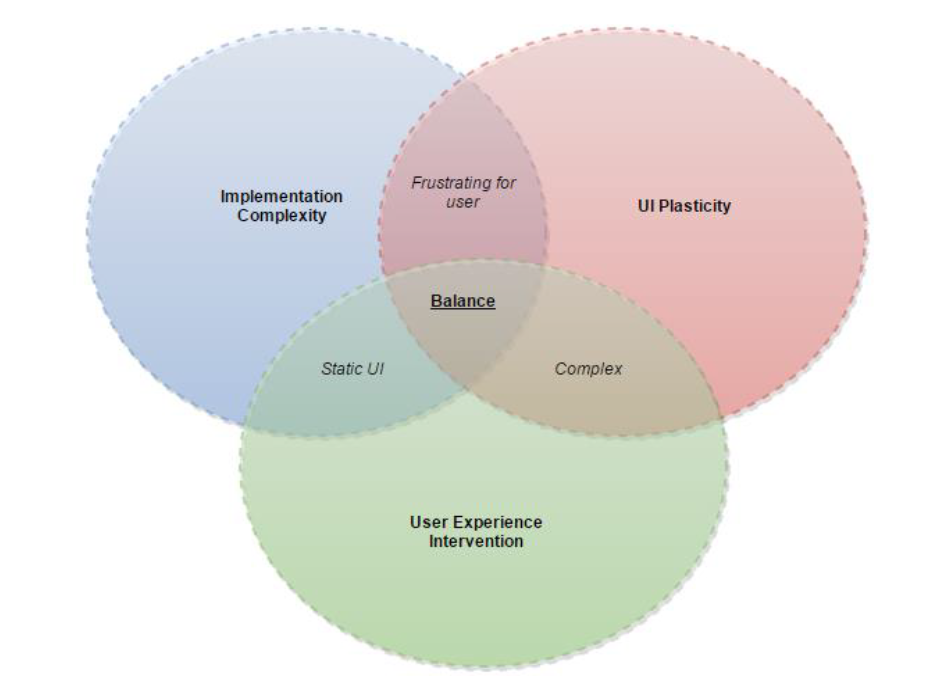
\includegraphics[height=.65\textwidth]{implChallenges.png}
    \caption{The three implementation challenges with the overlaps}
\end{figure}

\subsection{User experience intervention}
a UI with multiple adaptive components can cause unwanted interruptions to the user, and, in addition,
automatic and frequent adaptivity of interface may end up causing a feeling of loss of control [S. Kumar and A. Sekmen, "Single robot–Multiple human interaction via intelligent user interfaces," Knowledge-Based Systems, vol. 21, pp. 458-465, 2008.]

\textbf{Multiple adaptive components:} when the majority of the components that assemble the UI are
changing (irrelevant of the sophistication and excellence of the underlying intelligence in the adaptation decisions),
they can mess up with the user’s familiarity with the interface and take him out of his comfort zone.

Putting it into perspective, this indeed can spiral out of control and cause confusion,
stress and even frustration. It is really nice and elegant to have dropdown lists that add filter options when data input is large,
tables that sort themselves out based on input type, or pop-up windows that advise on next step and/or preselect actions for you; however,
if they all exist together and there are minimum standard UI components that can act as “reference points” for the user,
this can easily escalate into a bad experience for him and bring the adaptation effort to a failure.

\textbf{Simultaneous adaptation of components:} implementing behavior that changes the UI in an ad-hoc and disorderly mode can result
in a complete change of UI that will - at least! - confuse the user.

\textbf{User prompting:} Prompting the user for confirmation when filing in a password is a smart choice; also when he is about to overwrite a saved item,
or replace a UI component with a new one of his choice, or submitting a form etc. It is really important to point out that
this selection of UI components that will trigger prompting/confirmation has to be done in a very careful and user-centered way.
The line between facilitating and irritating pop-up windows is very thin and has to be taken under consideration while
implementing adaptation in runtime scenarios.

\subsection{Implementation Complexity}
Beim Erreichen von UI Adaptivität ist der dynamische, synchrone Wechsel der Benutzeroberfläche der komplizierteste Teil zu implementieren. 
In der Praxis muss das User Interface:
\begin{itemize}
    \item Die Daten und den Kontext zu jeder Zeit verstehen
    \item Sie mithilfe eines implementierten Entscheidungslogik prüfen
    \item Das UI und die adaptiven Komponenten auf einer effektiven, sanften und nicht blockierenden Art und Weise ändern
\end{itemize}

In the process of achieving UI adaptation, the part of real-time, dynamic changing of the UI (adaptivity) is arguably the
most complex part implementation-wise. In practice, the UI mechanism has to:
\begin{itemize}
    \item Understand the data and the context at any given time
    \item Evaluate them against the implemented logic of decision making
    \item Adapt the UI and its components in an effective, smooth and non task-blocking way
\end{itemize}

\subsection{Interface plasticity} %responsive web site = instance of a plastic user interface
Die dritte Herausforderung ist das Ergebnis der Adaptivität im User Interface. Diese Ergebnisse und deren Effekt auf den Nutzer 
können anhand ihrer "plasticity" gemessen werden.

\textbf{Plasticity}, zu deutsch (Ver-)Formbarkeit, wird benutzt, um die Leistungsfähigkeit des User Interfaces, 
Kontextwechsel der Nutzer standzuhalten und Änderungen der betroffenen Regionen zu adaptieren, 
um Benutzerfreundlichkeit zu gewährleisten.
"Therefore, in the context of a plastic UI, the goal is to maintain these properties within their values while achieving adaptation"
Zusammengefasst soll die Benutzeroberfläche:
\begin{itemize}
    \item effektiv,
    \item benutzbar,
    \item selbst-lernend,
    \item flüssig und
    \item benutzerfreundlich
\end{itemize}
sein, während sie sich dem Kontext anpasst. Das Komplexe am implementieren eines adaptiven UI ist der Sprung vom Abstrakten 
zu etwas Konkretem.
The third and equally important challenge that we come across is the actual result that the adaptation will bring to the User Interface.
These results, and the effect that they have, can be measured by the notion of plasticity.

\textbf{Plasticity} is a term that is interpreted in the bibliography in many (slightly) different variations,
although the root remains stable: it is the term used to describe the capacity of a user interface to withstand variations %Die Leistungsfähigkeit des User Interfaces, Kontextwechsel der Nutzer standzuhalten und Änderungen der betroffenen Regionen zu adaptieren, um Benutzerfreundlichkeit zu gewährleisten
of the context of use and adapt to changes of the interactive space in order to preserve usability [G. Calvary, J. Coutaz, D. Thevenin, Q. Limbourg, N. Souchon, L. Bouillon, et al., "Plasticity of user interfaces: A revisited reference framework" in In Task Models and Diagrams for User Interface Design, 2002.].
Therefore, in the context of a plastic UI, the goal is to maintain these properties within their values while achieving adaptation [L. Balme, A. Demeure, N. Barralon, J. Coutaz, and G. Calvary, "Cameleon-rt: A software architecture reference model for distributed, migratable, and plastic user interfaces" in Ambient intelligence, ed: Springer, 2004, pp. 291-302.].

In simple words, and as perceived under our research domain context, we want the user interface to be
1) effective,
2) usable,
3) self-learning,
4) fluid,
5) user-facilitating,
while adapting and changing based on the context. It should ideally resemble to the properties of plastic or brain:
learn, change and adapt to context changes with the purpose of improvement.
In terms of complexity, it is obviously a non-trivial task; aligning with generic notions of effectiveness and usability
while implementing and generating lines of coding is always a difficult task; this jump from abstract to concrete is
the main challenge of this type of problems.

\section{Themenabgrenzung}
Was wird aus inhaltlichen Gründen im Einzelnen untersucht oder aus umfangmäßigen Gründen nicht näher betrachtet. Ausführungen zur Untersuchungsmethodik.

\section{Motivation / Ziele}
Evaluation anhand eines Beispiels (Nutzerstudie)
\section{Firma}